\chapter{Propuesta}\label{chapter:proposal}

UTHOPIA propone un modelo de evaluación que sirve para comparar la inteligencia de humanos y la inteligencia de agentes de aprendizaje por refuerzo utilizando como base las premisas planteadas por Chollet (\cite{chollet2019measure}) y adicionalmente las conclusiones de los otros trabajos en entornos de evaluación de algoritmos de aprendizaje por reforzamiento. Brinda una interfaz para crear juegos que se centren en diferentes tareas que requieran habilidades de carácter cognitivo, cada una de las cuales pone a prueba un aspecto diferente del razonamiento. Aunque los supuestos prejuicios que planteamos son sencillos, al combinarlos podemos crear muchos problemas complejos que requieren la expresión de razonamiento cognitivo similar al humano.

Las características que se buscaron al construir UTHOPIA fueron:

\begin{itemize}
    \item Integrar evaluaciones tanto para humanos como para agentes con algoritmos de aprendizaje por reforzamiento.
    \item Centrarse en la medición de la generalización consciente del desarrollador (\ref{section:state-of-the-art:generalization-on-machine-learning}) en lugar de la habilidad específica, presentando únicamente tareas novedosas que se supone son desconocidas para el desarrollador del sistema.
    \item Medir de forma cualitativamente amplia la generalización, presentando tareas abstractas que deben ser comprendidas por el examinado con pocos ejemplos o tiempo para probar.
    \item Describir explícitamente el conjunto completo de prejuicios con los que cuenta y permitir una comparación de inteligencia general justa entre humanos y máquinas al requerir únicamente prejuicios cercanos al conocimiento previo humano innato.
\end{itemize}

\section{Prejuicios del conocimiento} 

Cualquier prueba de inteligencia va a implicar conocimientos previos. ARC trata de controlar sus propias suposiciones enumerando explícitamente el conocimiento previo que asume y evitando depender de cualquier información que no sea parte de este conocimiento previo (por ejemplo, el conocimiento adquirido como el lenguaje). Esto permite que el programa sea lo más cercano posible a los conocimientos previos innatos humanos, proporcionando un terreno justo para comparar la inteligencia artificial y la inteligencia humana, como recomendamos en (\ref{section:state-of-the-art:a-good-measure-of-inteligence:human-prios})

\textbf{Premisas de objetividad}
\begin{itemize}
\item Cohesión y delimitación de objetos: Definir las áreas que representan un objeto.
\item Persistencia de los objetos: Los objetos tienden a persistir en el juego al menos que se realice algún tipo de interacción explícita.
\item Influencia de los objetos a través del contacto: La mayoría de acciones se realizan mediante el contacto entre objetos.
\item Movimiento y dirección explícitos: La dirección y la movilidad de los objetos es deducible a partir de sus cambios de su posición en el tiempo.
\end{itemize}

\textbf{Números y capacidades de conteo}
\begin{itemize}
    \item Conteo de objetos ya sea que cumplen con similardad o determinadas propiedades dadas por las tareas.
\end{itemize}

\textbf{Conocimientos básicas de geometría y topología}
\begin{itemize}
\item Puntos, líneas y formas.
\item Similaridad entre objetos que por su color y forma se asocian al mismo tipo de función.
\item Simetrías, rotaciones y traslaciones.
\item Aumento o disminución de la forma, distorsiones de escala.
\item Contener, ser contenido y estar dentro o fuera de un perímetro.
\item Alcanzar o permanecer en el borde de un perímetro.
\item Superposición de objetos.
\end{itemize}

Como se ha sugerido en (\ref{section:state-of-the-art:a-good-measure-of-inteligence:human-prios}), no se incluye señales o símbolos cuya interpretación requiera conocimientos adquiridos tales como el lenguaje, números, señalamientos entre otros. 

\section{Estructura de UTHOPIA}

\begin{figure}[ht!]
    \centering
    \begin{subfigure}
      \centering
      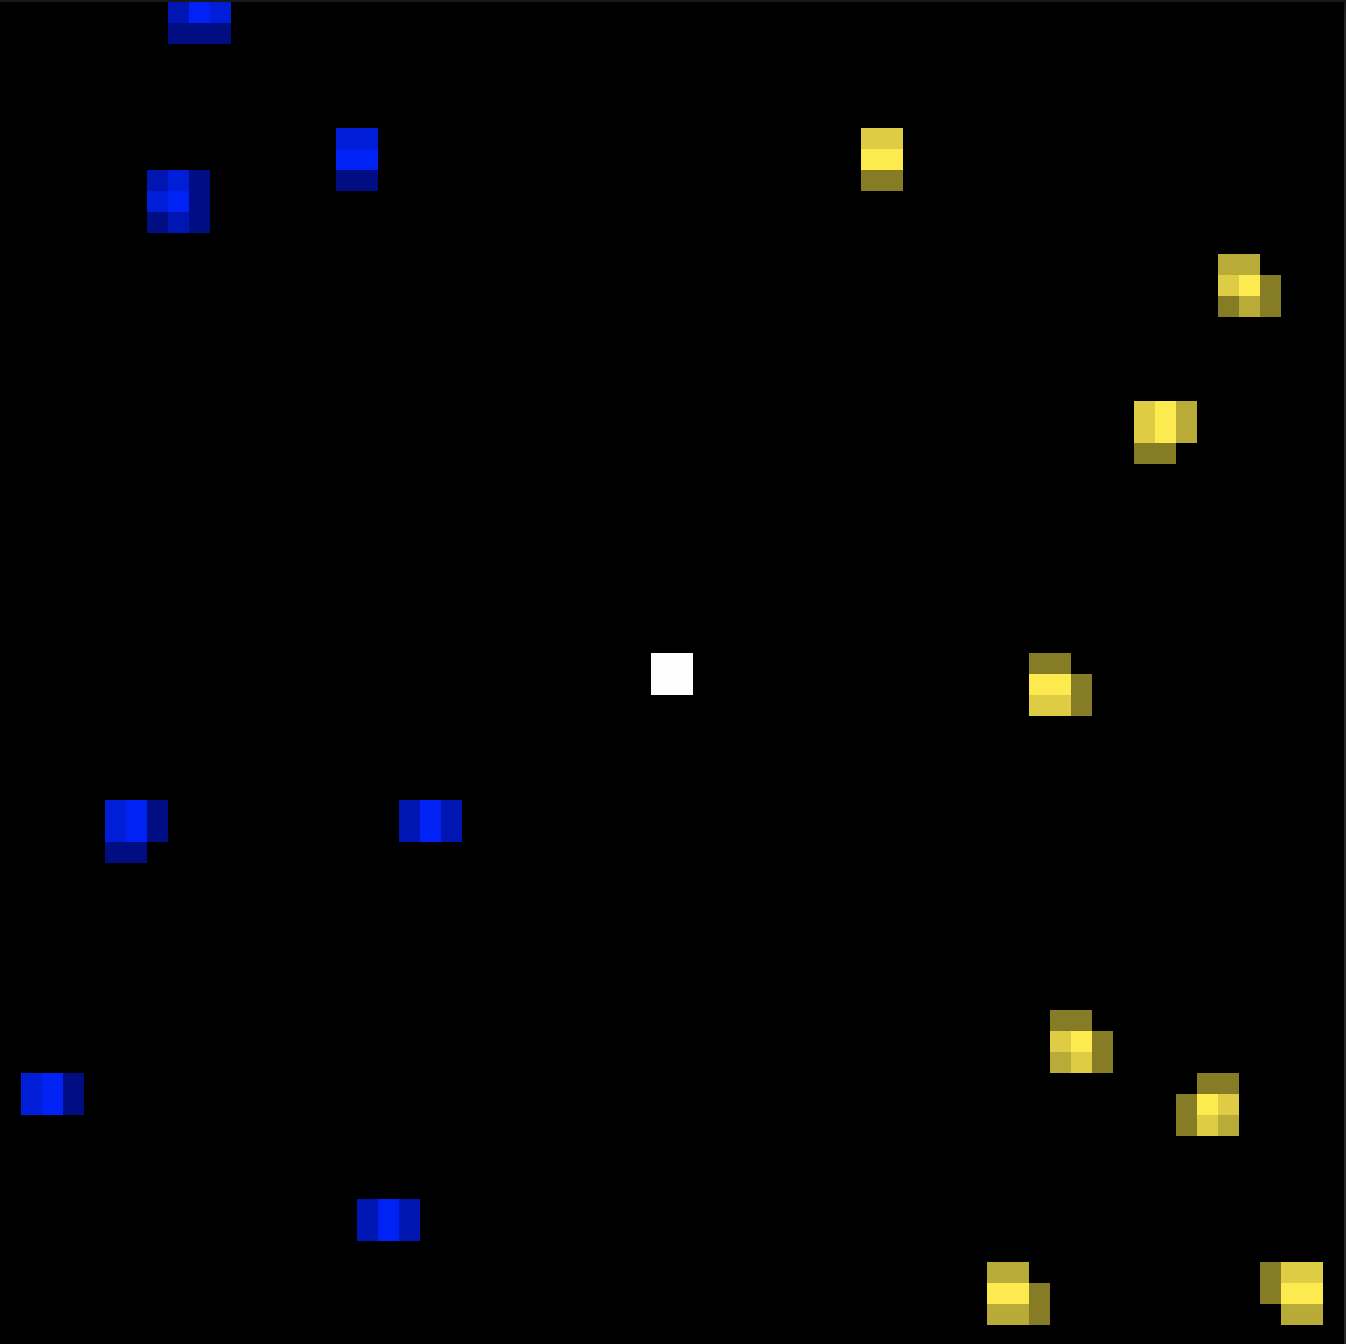
\includegraphics[width=0.4\textwidth]{Graphics/uthopia_count_war_1.png}
      \label{fig:uthopia1}
    \end{subfigure}%
    \begin{subfigure}
      \centering
      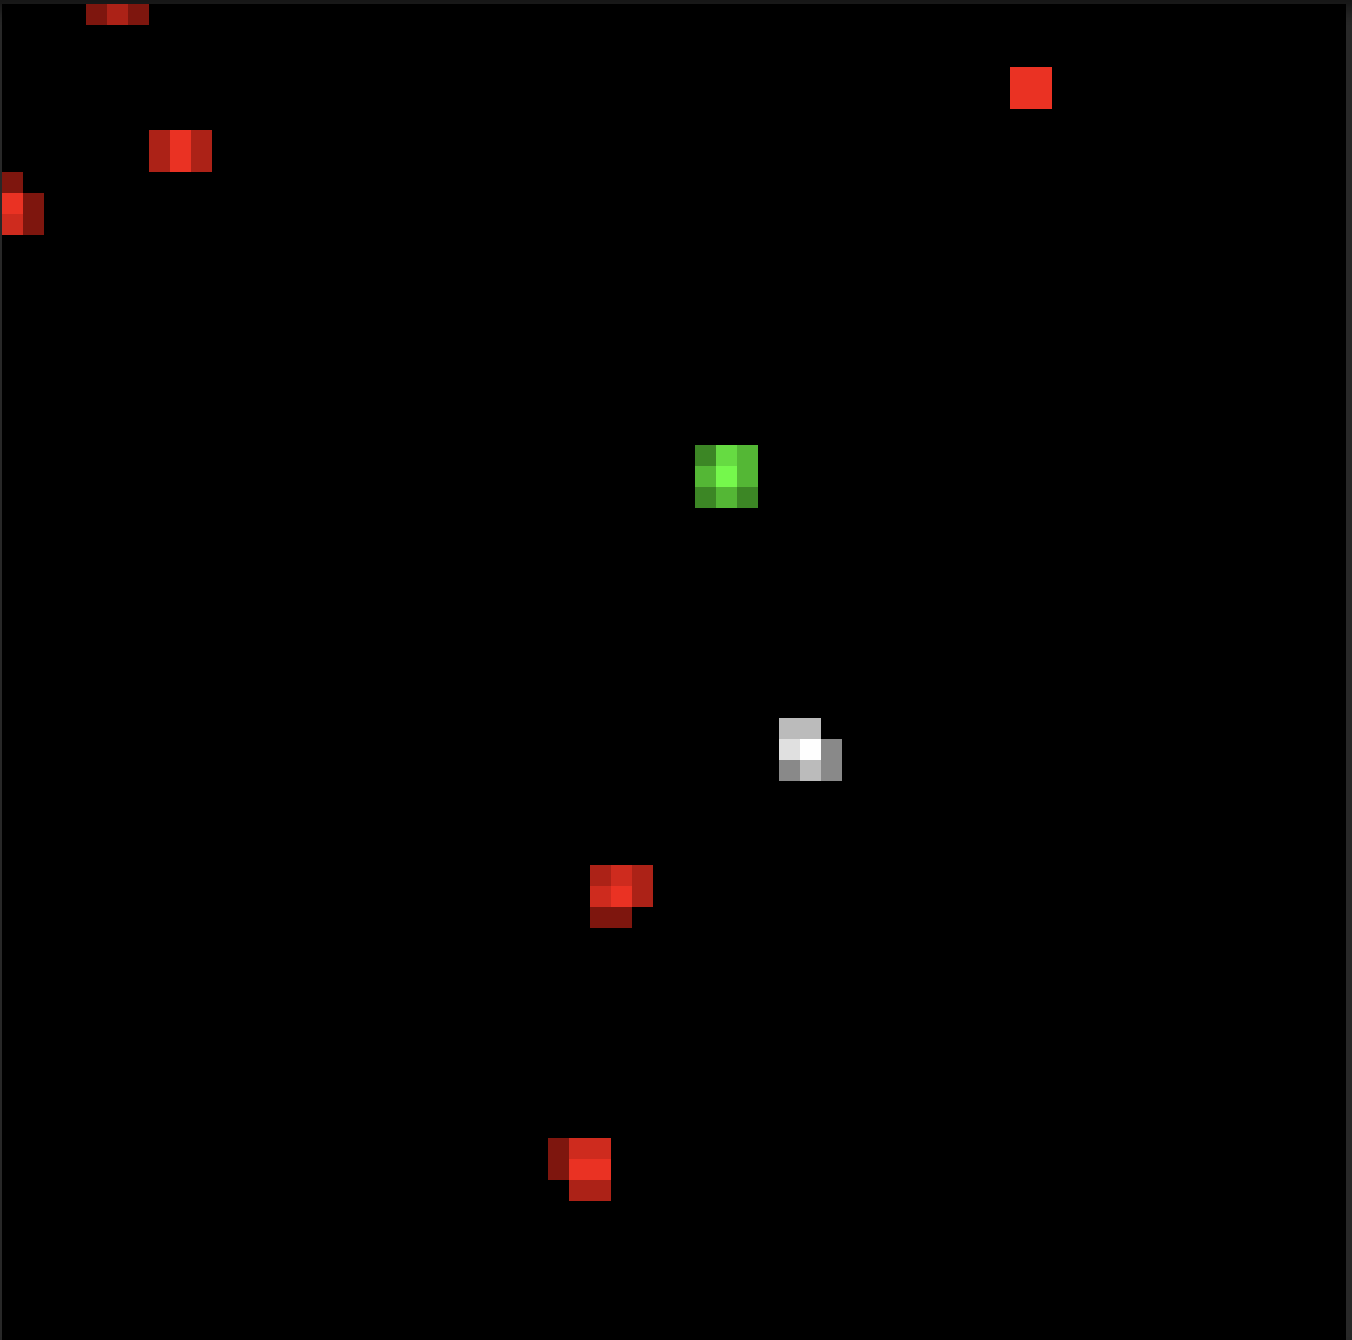
\includegraphics[width=0.4\textwidth]{Graphics/uthopia_evade_1.png}
      \label{fig:uthopia2}
    \end{subfigure}%
    \caption{Algunos juegos de UTHOPIA. A la izquierda elegir el bando con mayor numero y a la derecha tocar el objetivo evadiendo obstáculos.}
    \label{fig:uthopia}
\end{figure}

\begin{figure}[ht!]
    \centering
    \begin{subfigure}
      \centering
      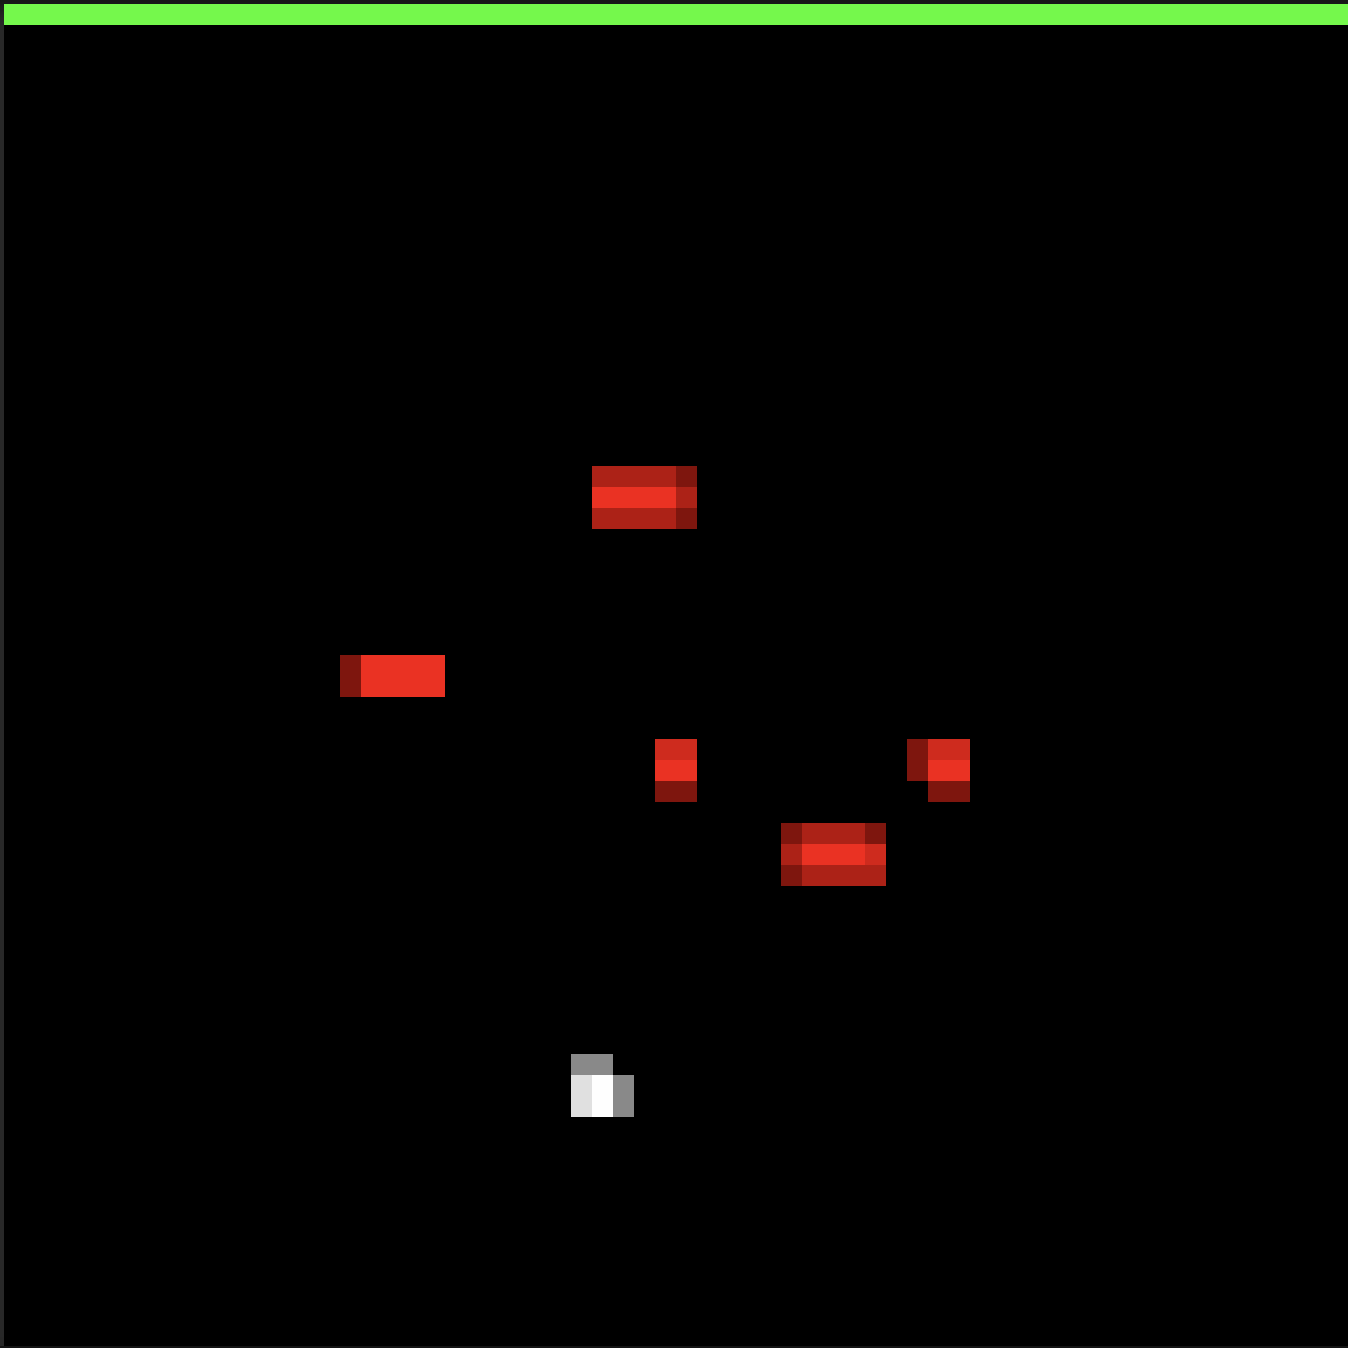
\includegraphics[width=0.4\textwidth]{Graphics/uthopia_street_1.png}
      \label{fig:uthopia_street_1}
    \end{subfigure}%
    \begin{subfigure}
      \centering
      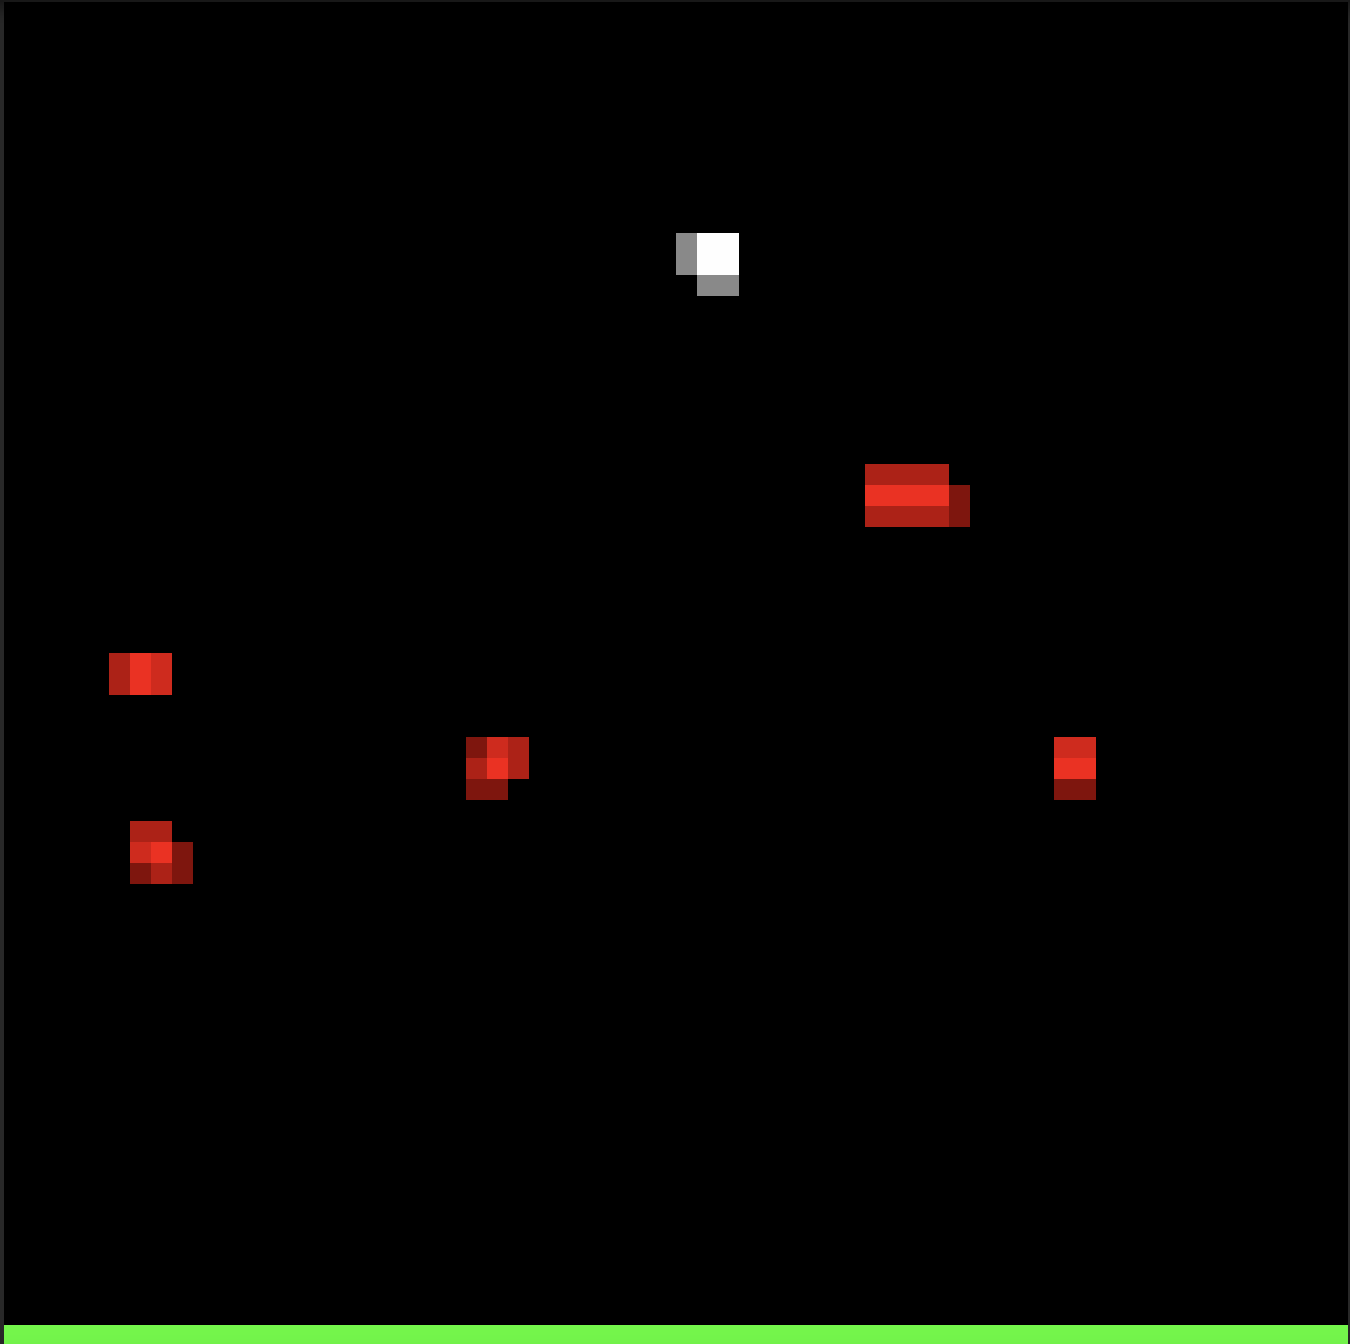
\includegraphics[width=0.4\textwidth]{Graphics/uthopia_street_2.png}
      \label{fig:uthopia_street_2}
    \end{subfigure}%
    \caption{Juego de cruzar. A la izquierda antes de alcanzar el primer objetivo y a la derecha luego de tocarlo}
    \label{fig:uthopia_street}
\end{figure}

\subsection{Características de los juegos}

Los juegos de UTHOPIA son simples (Fig \ref{fig:uthopia}). El objetivo de cada uno es capturar elementos del razonamiento cognitivo. Se intenta retirar todos los factores distractores que no tengan peso en el significado abstracto de la tarea evaluada. Cada juego está formado por objetos de color entero y con formas simples. Su interacción ocurre mediante el contacto entre ellos. No es necesario jugar de forma óptima para terminar los juegos correctamente, y en su mayoría la dificultad es ajustable. Se ha intentado, además, que todos los juegos tengan solución en cada episodio. 

Para brindar experiencias que no lleven a los agentes a sobre ajustarse se ejecuta en cada episodio de juego la regeneración del estado inicial de forma procedural.

\subsection{Configuración del aprendizaje por refuerzo}

Desde la perspectiva del aprendizaje por refuerzo para un solo agente definimos las observaciones, las acciones y las recompensas de la siguiente manera:

\begin{itemize}
    \item Observaciones: Una única cámara que muestra una cuadrícula de píxeles con resolución $K * K * 3$ donde $32 \eqslantless K \eqslantless 256$.
    \item Espacio de acción: El agente puede tomar hasta $8$ acciones, de ellas las primeras $4$ indican dirección de forma semántica, cuyo efecto concreto dentro del juego puede variar según se diseñe. Tanto las acciones de dirección como las restantes pueden ser o no válidas para todos los juegos, por eso en cada uno se especificará explícitamente las acciones aceptadas.
    \item Señal de Recompensa: Cada juego tiene una evaluación binaria. Las recompensas están dadas por la terminación correcta o incorrecta de los mismos. Cada juego tiene asociado una cantidad máxima de tiempo de juego, luego de este el juego termina fallido.
\end{itemize} 

\subsection{El flujo de evaluación para agentes inteligentes en UTHOPIA}\label{chapter:proposal:evaluation-flow}

\begin{figure}[ht!]
    \centering
    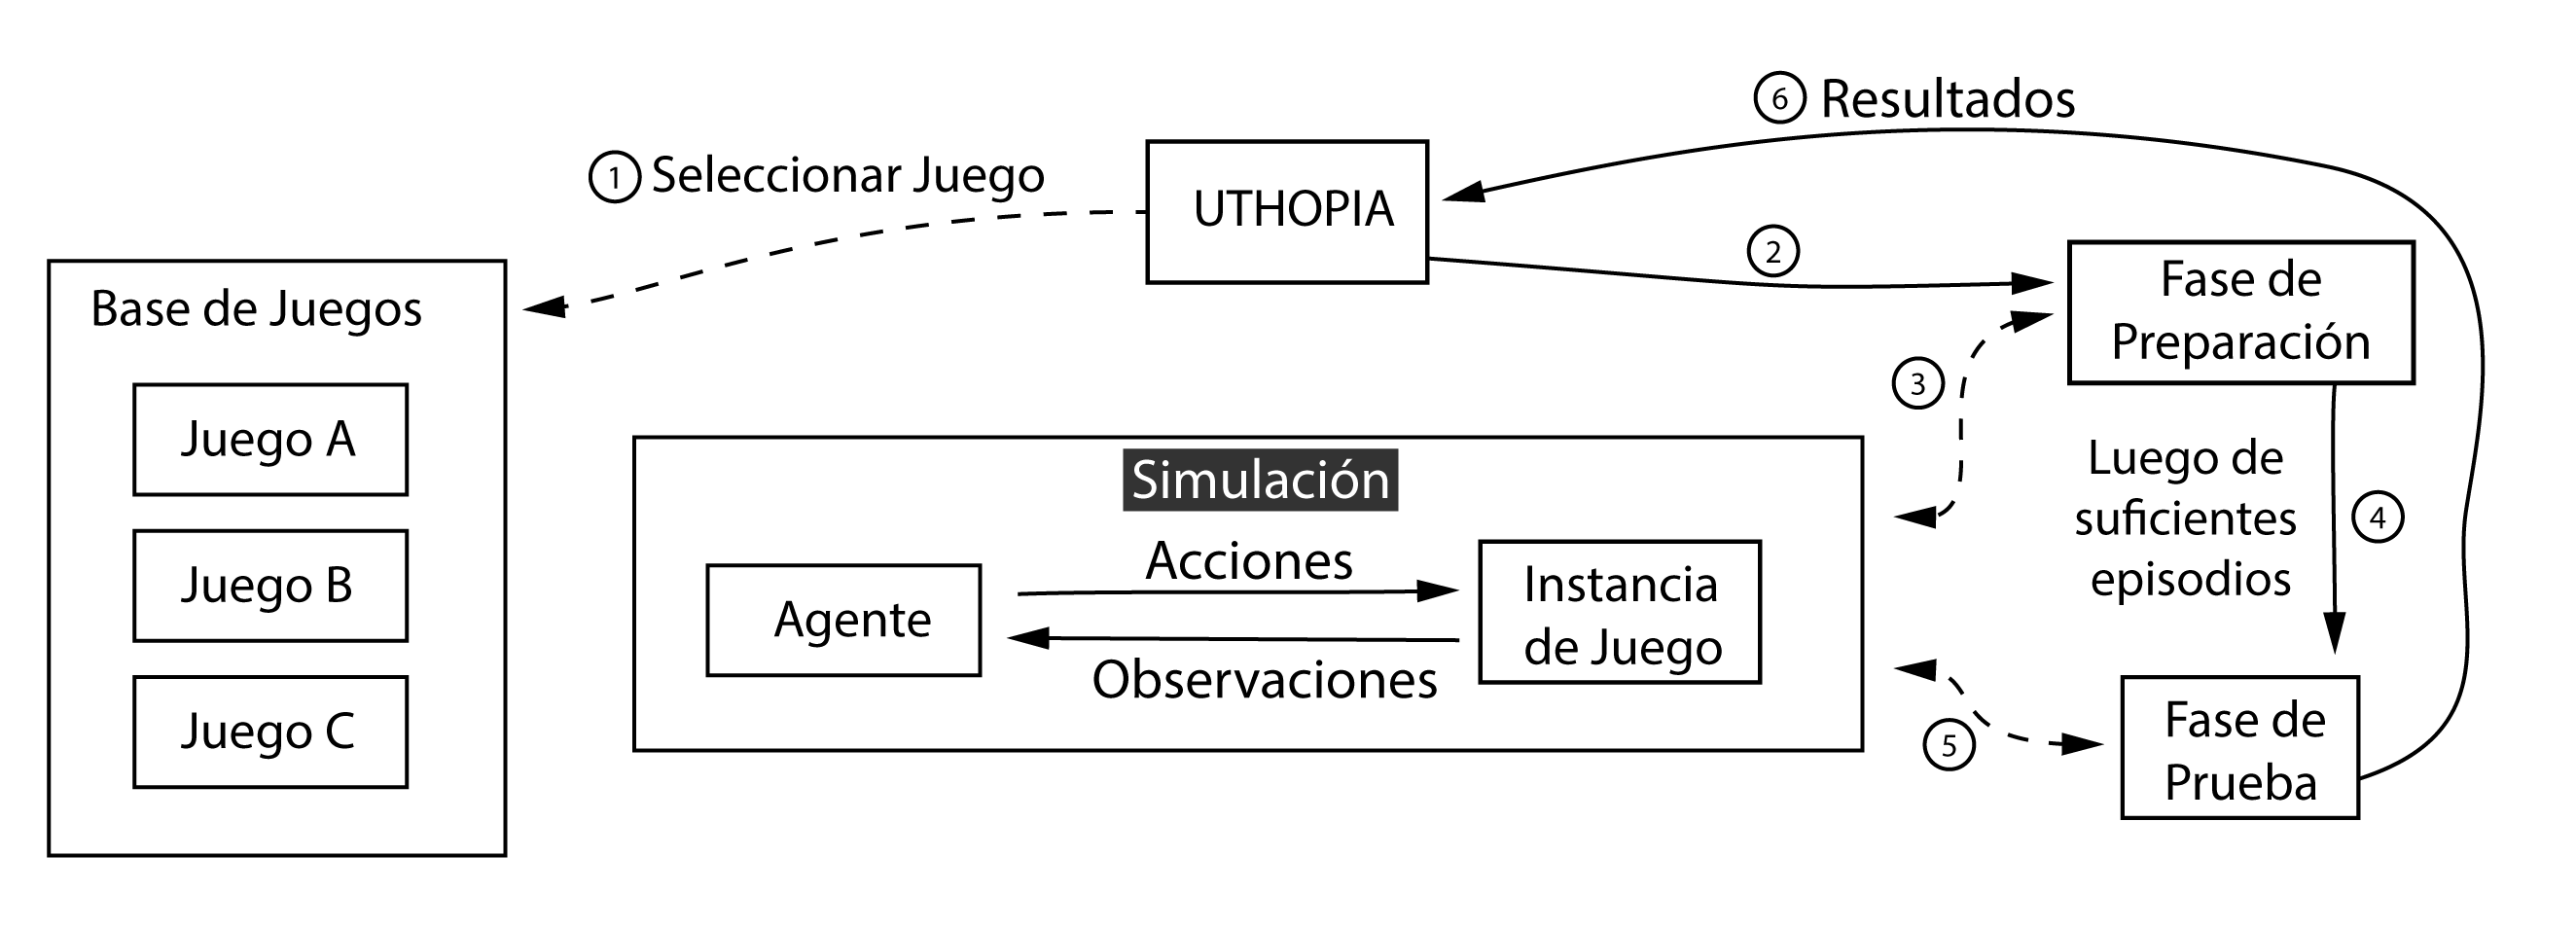
\includegraphics[width=0.9\textwidth]{Graphics/uthopia_flow.png}
    \caption{Diagrama de flujo de la evaluación en UTHOPIA.}
    \label{fig:uthopia_flow}
\end{figure}

El primer paso en el proceso de evaluación consiste en seleccionar uno de los juegos de la base de juegos creados, de esos un conjunto son públicos y el resto se reserva para la evaluación privada de aquellos que apliquen intentando evaluar la generalización consciente del desarrollador (\ref{section:state-of-the-art:generalization-on-machine-learning:type-of-generalizations}). El orden de selección se hace en base al estimado de dificultad de generalización que presenta cada uno, tratando de aumentar la dificultad de forma gradual.

Una vez se ha seleccionado el juego comienza el primer episodio de la \textit{Fase de Preparación}. Durante la esta etapa UTHOPIA crea continuamente instancias del juego para que el agente se familiarice y capte la esencia detrás de la tarea cognitiva que la resuelve. Se expone a episodios del juego durante un tiempo determinado relativamente corto (comparado al entrenamiento habitual que reciben los algoritmos de aprendizaje por reforzamiento) algo mayor al que un humano promedio necesitaría para entender la tarea.

Pasada la fase de preparación se procede a la \textit{Etapa de Prueba} donde se crean nuevas instancias del mismo juego seleccionado utilizando otras semillas para la generación. Esta vez se evalúa la solución las tareas. El resultado cada episodio es binario y los agentes se consideran aprobados si resuelven correctamente la tarea en un número suficiente de intentos.

Luego de realizar la prueba sobre toda la batería de juegos se da a conocer el resultado de inteligencia. En este punto la comparativa de los resultados de los agentes humanos constituye el principal recurso utilizado para valorar el rendimiento de los agentes de inteligencia artificial.



